% \begin{columns}[onlytextwidth]
%     \begin{column}{0.5\textwidth}
%     \end{column}
%     \begin{column}{0.5\textwidth}
%     \end{column}
% \end{columns}

\section{Part 3: Statistics and Probability}
\subsection{Random Variables}

{
    \small

    \begin{frame}{Introduction}
        Background
        \begin{itemize}
            \item Probability is the mathematical field concerned with reasoning under uncertainty
            \item Probabilistic models enable us to reason about the \emph{likelihood} of various events
            \item Use of probabilities to describe the frequencies of repeatable events
                  (like coin tosses) is fairly uncontroversial
        \end{itemize}

        Schools of thoughts
        \begin{itemize}
            \item Frequentists scholars adhere to an interpretation of probability that applies only to such repeatable events
            \item Bayesian scholars use the language of probability more broadly to formalize our reasoning under uncertainty
        \end{itemize}

        Bayesian probability is characterized by two unique features:
        \begin{itemize}
            \item assigning prior belief e.g., $P[\text{"moon is made out of cheese"}]$, opions may differ
            \item evidence, that is hard facts that we measure
        \end{itemize}
        Bayesian probability provides unambiguous rules for how we should \emph{update} our belief in light
        of new evidence, while allows for different individuals to start off with different prior beliefs
    \end{frame}

    \begin{frame}{Terminology}
        Imagine the experiment:
        \begin{itemize}
            \item Toss a coin $n$ times. The probability for heads is $p_h = 1/2$.
            \item We observe $n_h$ heads and $n_t = n - n_h$ tails
            \item Fraction of heads that we \emph{expect} to see should exactly match the expected fraction of tails
            \item The larger $n$ the less likely $n_h = n_t$ becomes
        \end{itemize}

        Terminology:
        \begin{itemize}
            \item $p_h$ is called a \emph{probability}, captures the certainty with which any given toss will come up heads
            \item Probabilities assign scores between $0$ and $1$ to \emph{events} (i.e. the outcomes of interest)
            \item Here the event of interest is ``heads'' and we denote the corresponding probability $P(\text{heads})$
            \item $P(\cdot) = 1$ indicates absolute certainty, and $P(\cdot) = 0$ impossibility
            \item $n_h / n$ and $n_t / n$ are called \emph{statistics} (not probabilities)---empirical quantities
                  computed based on the observed data
            \item \emph{Estimators} are special statistics that use the data to produce estimates of model parameters (like probabilities).
                  \emph{Consistent estimators} converge to the corresponding probability (cf. next slide)
        \end{itemize}
    \end{frame}

    \begin{frame}
        \vspace*{5mm}
        Estimators and Consistency
        \begin{center}
            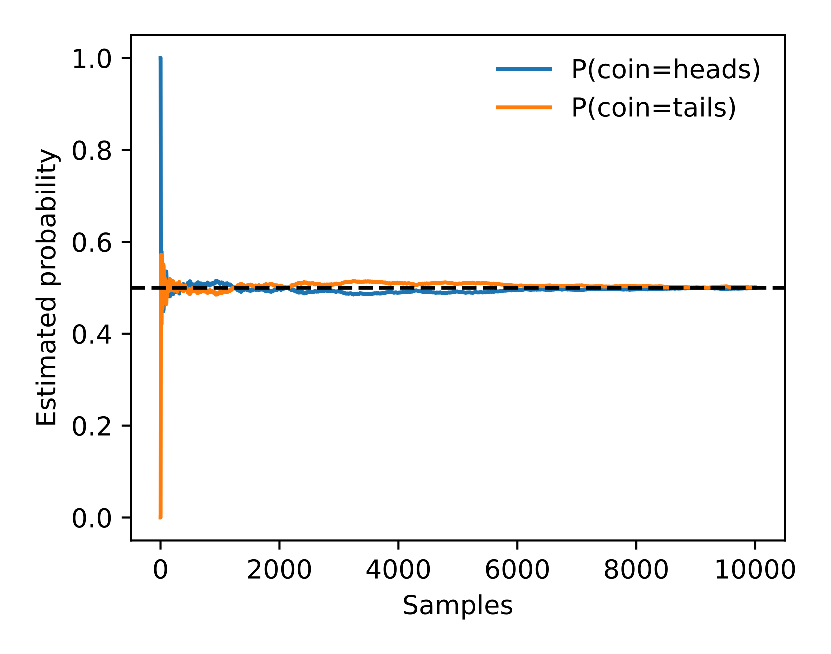
\includegraphics[width=0.6\textwidth]{fig/prob_estimator_convergence.eps}
        \end{center}
    \end{frame}

    \begin{frame}{Formal Definition}
        Denote the set of possible outcomes $\mathcal{S}$, and call it the \emph{sample space} or \emph{outcome space}, e.g.:
        \begin{itemize}
            \item Rolling a single coin: $\mathcal{S} = \{\textrm{heads}, \textrm{tails}\}$
            \item Rolling a single die, $\mathcal{S} = \{1, 2, 3, 4, 5, 6\}$
            \item flipping two coins, possible outcomes are
                  $\{(\textrm{heads}, \textrm{heads}), (\textrm{heads}, \textrm{tails}), (\textrm{tails}, \textrm{heads}),  (\textrm{tails}, \textrm{tails})\}$
        \end{itemize}
        \emph{Events} are subsets of the sample space.

        \begin{boxed}
            \textbf{Axioms of Probability}:
            A \emph{probability function} maps events onto real values
            ${P: \mathcal{A} \subseteq \mathcal{S} \rightarrow [0,1]}$.
            The probability of an event $\mathcal{A}$ in the given sample space $\mathcal{S}$, denoted $P(\mathcal{A})$,
            satisfies the following properties (Kolmogorov, 1933):

            \begin{itemize}
                \item The probability of any event $\mathcal{A}$ is a non-negative real number, i.e., $P(\mathcal{A}) \geq 0$;
                \item The probability of the entire sample space is $1$, i.e., $P(\mathcal{S}) = 1$;
                \item For any countable sequence of events $\mathcal{A}_1, \mathcal{A}_2, \ldots$ that are \emph{mutually exclusive} ($\mathcal{A}_i \cap \mathcal{A}_j = \emptyset$ for all $i \neq j$), the probability that any of them happens is equal to the sum of their individual probabilities, i.e., $P(\bigcup_{i=1}^{\infty} \mathcal{A}_i) = \sum_{i=1}^{\infty} P(\mathcal{A}_i)$.
            \end{itemize}
        \end{boxed}
    \end{frame}



    \begin{frame}{Random Variables}
        A \emph{random variable} (RV) is a mapping from an underlying sample space to a set of values
        \begin{itemize}
            \item Random variables can be much coarser than the raw sample space. E.g. define RV
                  ``greater than 0.5'' is binary but has an infinite sample space
            \item Multiple RVs may share the same underlying sample space. E.g. for RVs ``home alarm goes off''
                  and ``my house was burglarized'', knowing the value taken by one random variable can tell us
                  something about the likely value of another random variable
        \end{itemize}

        Every value taken by a random variable corresponds
        to a subset of the underlying sample space.
        Thus the occurrence where the random variable $X$
        takes value $v$, denoted by $X=v$, is an \emph{event}
        and $P(X=v)$ denotes its probability.
    \end{frame}

    \begin{frame}
        Notation in practice
        \begin{itemize}
            \item $P(X)$ may refer broadly to the \emph{distribution} of $X$
            \item $P(X,Y) = P(X) P(Y)$, may be shorthand to express a statement
                  that is true for all of the values
                  that the random variables $X$ and $Y$, i.e.,
                  $\forall i,j : P(X=i \textrm{ and } Y=j) = P(X=i)P(Y=j)$
            \item $P(v)$ may be used when the random variable is clear from the context
            \item $P(1 \leq X \leq 3)$ may denote the probability of the event $\{1 \leq X \leq 3\}$
        \end{itemize}

        In general, there's two types of random variables:
        \begin{itemize}
            \item Discrete, e.g. flips of a coin or tosses of a die
            \item Continuous, e.g. height $H$ of a person. Note that in this case, asking e.g.
                  for $P(H = 1.8796549851915233234)$ does not make sense. Instead, we work with
                  probability \emph{densities} p
        \end{itemize}

    \end{frame}

    %   \begin{frame}{// additional}
    %       \url{http://d2l.ai/chapter_preliminaries/probability.html#multiple-random-variables}

    %       \url{http://d2l.ai/chapter_preliminaries/probability.html#expectations}
    %   \end{frame}

    \subsection{Density and Distribution Functions}

    \begin{frame}{Probability Density Functions (PDFs)}
        \begin{columns}[onlytextwidth]
            \begin{column}{0.55\textwidth}
                \begin{boxed}
                    \textbf{PDF}:
                    Informally, a PDF $p(x)$ is characterized by the following properties:
                    \begin{itemize}
                        \item ${\displaystyle p(x) \geq 0 }$
                        \item ${\displaystyle \int_{-\infty}^{\infty} p(x)  \d x = 1 }$
                    \end{itemize}
                    From this it follows that the probability of any single value $x$
                    is $0$, $P(X = x) = 0$ and that $p(x) > 1$ is admissible
                \end{boxed}

                To compute actual probabilities we integrate $p(x)$ over an \emph{interval}:
                $$P(X\in(a, b]) = \int _ {a}^{b} p(x) \d x$$
            \end{column}
            \begin{column}{0.45\textwidth}
                \centering
                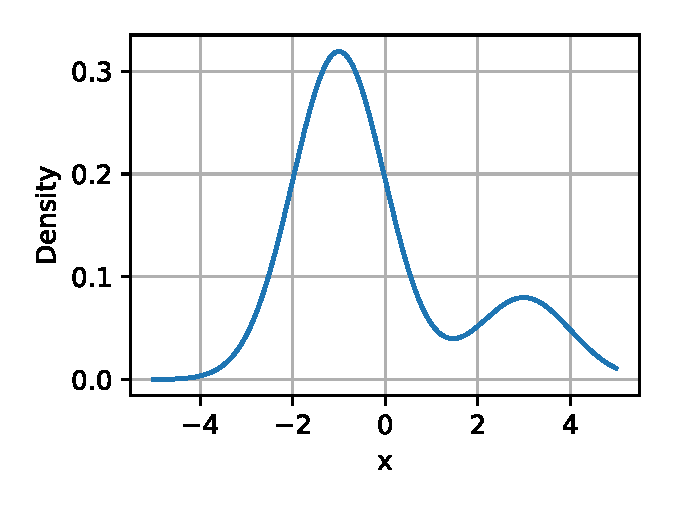
\includegraphics[width=0.70\textwidth]{fig/prob_density_1.eps}
                \hspace*{2mm}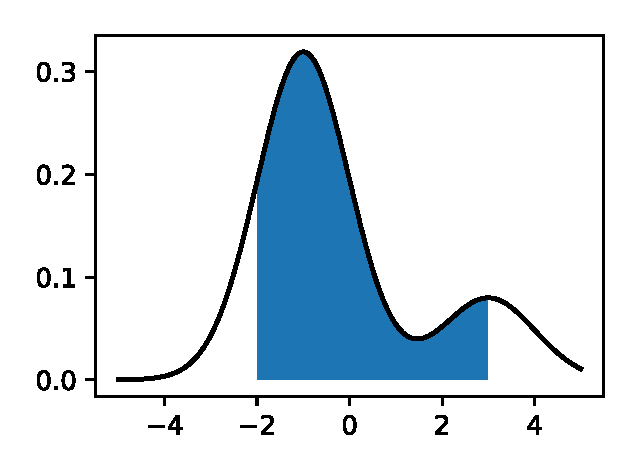
\includegraphics[width=0.65\textwidth]{fig/prob_density_2.eps}
            \end{column}
        \end{columns}
    \end{frame}

    \begin{frame}{Cumulative Distribution Functions (CDFs)}
        \begin{boxed}
            The CDF $F(x)$ of a random variable $X$ with density $p(x)$ is given by
            $$F(x) = \int _ {-\infty}^{x} p(x) \d x = P(X \le x)$$
            Note that $F(x)$ represents an actual probability
        \end{boxed}

        Properties:
        \begin{itemize}
            \item $F(x) \rightarrow 0$ as $x\rightarrow -\infty$
            \item $F(x) \rightarrow 1$ as $x\rightarrow \infty$
            \item $F(x)$ is non-decreasing, i.e. $y > x \implies F(y) \ge F(x)$
            \item $F(x)$ is continuous (has no jumps) if $X$ is a continuous random variable
        \end{itemize}
    \end{frame}

    \begin{frame}{Characterizing Distributions}
        \framesubtitle{Expected value}
        \begin{boxed}
            \textbf{Expected value of a RV (mean)}:
            \begin{itemize}
                \item $\displaystyle \mu_X = \E X = \sum_i x_i\,p_i \quad \text{(for discrete RV $X$)}$
                \item $\displaystyle \mu_X = \E X = \int_{-\infty}^\infty x\,p(x) \d x \quad \text{(for continuous RV $X$)}$
            \end{itemize}
        \end{boxed}

        Properties:
        \begin{itemize}
            \item For any RV $X$ and numbers $a$ and $b$, we have that $\mu_{aX+b} = a\mu_X + b$
            \item For any two random variables $X$ and $Y$, we have $\mu_{X+Y} = \mu_X+\mu_Y$
        \end{itemize}

        Means characterize average behavior of a RV, which is not sufficient however:
        A profit of $CHF 10 \pm CHF 1$ per sale is very different from making $CHF 10 \pm CHF 15$ per sale.
    \end{frame}

    \easterchallenge{
        One possibility to quantify risk $r$ as expected loss. That is, by weighting the loss $l$ (e.g., in CHF)
        which some event causes with the probability $p_e$ that this event actually occurs:
        $$r := p_e\:l$$

        Now assume you want to park your car in the city of Zurich. The parking garage will charge you CHF 24.
        If you park in some quiet corner, you may get fined and pay CHF 40. The chance that you'll get caught is $2/3$.
        What's the rationale choice here, parking garage or taking your chances?
    }{
        The parking garage as it has the lower expected loss: $24 < \frac 2 3 \times 40 \approx 26.67$
    }

    \begin{frame}{Characterizing Distributions}
        \framesubtitle{Variance and Standard Deviation}

        \begin{boxed}
            \textbf{Variance}:
            The variance measures the variation of a RV about its mean:
            $$\sigma_X^2 = \mathrm{Var}(X) = E\left[(X-\mu_X)^2\right]$$
        \end{boxed}

        Properties:
        \begin{itemize}
            \item For any RV $X$, $\mathrm{Var}(X) \ge 0$, with $\mathrm{Var}(X) = 0$ iff $X$ constant
            \item For any RV $X$ and numbers $a$ and $b$, we have that $\mathrm{Var}(aX+b) = a^2\mathrm{Var}(X)$
            \item For any two independent RV $X$ and $Y$, we have $\mathrm{Var}(X+Y) = \mathrm{Var}(X) + \mathrm{Var}(Y)$
            \item $\displaystyle E\left[(X-\mu_X)^2\right] = E[X^2] - \mu_X^2$
        \end{itemize}

        \begin{boxed}
            \textbf{Standard Deviation (SD)}:
            The SD also measures  the variation of a RV about its mean, but has the same units as the mean:
            $$\sigma_X = \sqrt{\mathrm{Var}(X)}$$
        \end{boxed}
        Analogous properties as in the case of variance apply
    \end{frame}

    \begin{frame}{Continuous Distributions}
        \framesubtitle{A Well Behaved Example}

        Task: Compute the first two moments of the uniform distribution
        $$
            p(x) = \begin{cases}
                1 & x \in [0,1],     \\
                0 & \text{otherwise}
            \end{cases}
        $$
        \vspace*{5mm}

        Find expected value:
        $$\mu_X = \int_{-\infty}^\infty xp(x) \d x = \int_0^1 x \d x = \frac{1}{2}$$

        Find variance:
        $$\sigma_X^2 = \int_{-\infty}^\infty x^2p(x) \d x - \left(\frac{1}{2}\right)^2
            = \frac{1}{3} - \frac{1}{4} = \frac{1}{12}
        $$
        where we used above identity $\E{(X-\mu_X)^2} = \E {X^2} - \mu_X^2$
    \end{frame}

    \begin{frame}{Continuous Distributions}
        \framesubtitle{An Less Well-Behaved Example}

        \begin{columns}[onlytextwidth]
            \begin{column}{0.55\textwidth}
                Task: Compute the first two moments of a Cauchy-like distribution with the PDF given by
                $$p(x) = \frac{1}{1+x^2}$$
                \vspace*{3mm}

                Trying to compute the variance yields
                $$\sigma_X^2 = \int_{-\infty}^\infty x^2p(x) \d x
                    = \int_{-\infty}^\infty \frac{x^2}{1+x^2} \d x = \infty
                $$
                Hence the variance of $p(x)$ is undefined.\\[3mm]

                A similar problem arises for the mean, which is undefined too.
            \end{column}
            \begin{column}{0.45\textwidth}
                \begin{center}
                    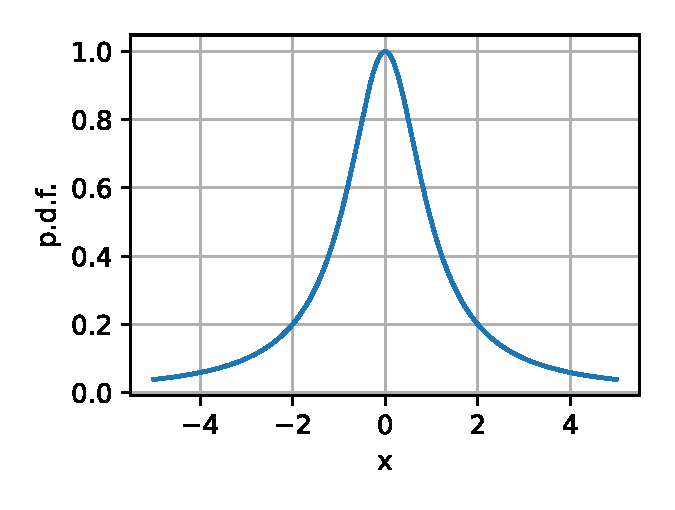
\includegraphics[width=0.85\textwidth]{fig/prob_cauchy.eps}
                \end{center}
            \end{column}
        \end{columns}


    \end{frame}

    \subsection{Joint, Marginal, and Conditional Densitities}

    \begin{frame}{Joint Density}
        Similar to the univariate case, a PDF can be defined for two or more variables.

        The two RVs $X$ and $Y$ can be defined to have a \emph{joint density} $p(x, y)$ or $p_{X, Y}$.
        Then properties similar to the univariable case hold:
        \begin{itemize}
            \item $\displaystyle p(x, y) \ge 0$
            \item $\displaystyle \int _ {\mathbb{R}^2} p(x, y) \d x \d y = 1$
            \item $\displaystyle P((X, Y) \in \mathcal{D}) = \int _ {\mathcal{D}} p(x, y) \d x \d y$
        \end{itemize}

        This generalizes to any number of RVs.
    \end{frame}

    \begin{frame}{Marginal Distributions}
        When dealing with multiple variables, we often ask ``how is this one variable distributed?''.
        The distribution that answers this questions this is the \emph{marginal distribution}.

        Mathematically (often referred to as \emph{integrating out} or \emph{marginalizing out} unneeded variables):
        $$p _ X(x) = \int_{-\infty}^\infty p_{X, Y}(x, y) \d y$$

        Visually:
        \begin{center}
            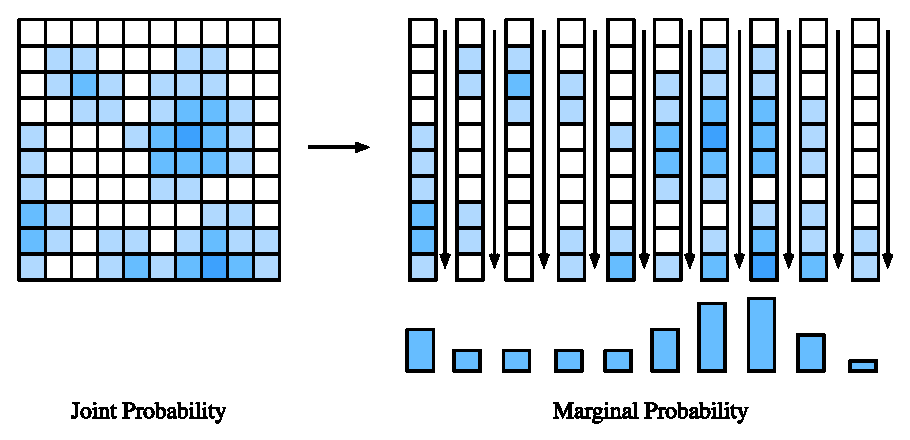
\includegraphics[width=0.6\textwidth]{fig/prob_marginal_distr.eps}
        \end{center}
    \end{frame}

    \begin{frame}{Conditional Probability and Statistical  Independence}
        The conditional distribution quantifies the probability of an event occurring,
        given that another event (e.g. by assertion or by evidence) has already occurred.

        \begin{boxed}
            \textbf{Conditional Probability}:
            We define the conditional probability of ``$\ev A$ given $\ev B$'', written $P(\ev A \mid \ev B)$ to be:
            $$P(\ev A \mid \ev B) = \frac{P(\ev A, \ev B)}{P(\ev B)}
                \quad \text{or equivalently} \quad
                P(\ev A, \ev B) = P(\ev A \mid \ev B) \, P(\ev B)$$
        \end{boxed}

        Based on the above we define independence:

        \begin{boxed}
            \textbf{Statistical Independence}:
            Events $\ev A$ and $\ev B$ are defined to be \emph{statistically independent} if
            $$P(\ev A, \ev B) = P(\ev A) \, P(\ev B)$$
        \end{boxed}

        Therefore independence implies both $P(\ev A \mid \ev B) = P(\ev A)$ and $P(\ev B \mid \ev A) = P(\ev B)$
    \end{frame}

    \begin{frame}{Conditional Independence}
        % \vspace*{2mm}        
        Conditional probabilities are proper probabilities $\Rightarrow$ concepts of (in)dependence also apply to them.

        \begin{boxed}
            \textbf{Conditional Independence}:
            Two RVs $A$ and $B$ are \emph{conditionally independent} given a third RV $C$ iff
            $$P(A, B \mid C) = P(A \mid C) \: P(B \mid C)$$
        \end{boxed}

        Two independent RV can become dependent when conditioning on a third RV $C$.
        Occurs when RVs $A$ and $B$ correspond to causes of RV $C$.

        Example:
        \begin{itemize}
            \item A broken bone and lung cancer might be independent in the general population
            \item Now condition on being in the hospital
            \item Conditionally, the broken bone is negatively correlated with lung cancer
            \item We say the broken bone \emph{explained away} why some person is in the hospital,
                  in turn lowering the probability that the person has lung cancer
        \end{itemize}
    \end{frame}


    \begin{frame}{Bayes' Theorem}
        By definition of conditional probabilities, $P(A, B) = P(B\mid A)\:P(A)$ and
        $P(A, B) = P(A\mid B)\:P(B)$,
        which is equivalent to
        \begin{boxed}
            \textbf{Bayes' Theorem}:
            $$P(A \mid B) = \frac{P(B\mid A)\:P(A)}{P(B)}$$
        \end{boxed}

        Please note the profound implications: It allows us to reverse the order of conditioning. If
        we know how to estimate $P(B\mid A)$, $P(A)$, and $P(B)$, then we can estimate $P(A\mid B)$.

        Example:\\
        Given  the prevalence of symptoms for a given disease,
        and the overall prevalences of the disease and symptoms, respectively,
        we can determine how likely someone is to have the disease based on their symptoms.

        Special case: Without direct access to $P(B)$, we still know that
        $$P(A \mid B) \propto P(B \mid A) P(A)$$
        and use the normalization constraint $\sum_a P(A=a \mid B) = 1$.

    \end{frame}

    \begin{frame}{Marginalization}
        Marginalization (``sum rule'') is key ingredient to make Bayes theorem work.

        It simply sums or integrates out, respectively, other variables from the joint distribution:
        $$P(B) = \sum_a P(A, B)$$
        $$p_B = \int_{-\infty}^{\infty} p(a,b)\d a$$

        The result is called marginal probability.

        In practice, where joint probabilities consist of many variables, this ``normalizer'' term
        in Bayes' theorem often becomes a computational bottleneck.
    \end{frame}

    \easterchallenge{
        It's 1963 and you participate in ``Let's Make a Deal'' (TV Show). You play this game:
        \begin{itemize}
            \item There's three doors: behind two of them there's a goat, behind the third a Ferrari
            \item First you pick a door
            \item Then the host opens one of the two other doors with a goat behind
            \item Then you can optionally switch to the other closed door or stay with your initial one
            \item Then your door will be opened and if it's the Ferrari, the car is yours
        \end{itemize}
        If you want the car, what's best to do? a) stay, b) switch, c) makes no difference\\
        Hint: Use Python or Bayes' theorem
    }{
        With loss of generality, you pick door 1 and the host opens door 2 or 3. Let $D := \text{``number of the door with the car behind''} \in \{1,2,3\}$,
        and likewise $H := \text{number of door which host opens}$. At the end of the game there's two options, $d=1$ and $d=3$:\\
        $$P(D = d \mid H = 2) = \frac{P(H = 2 \mid D = d)\, P(D = d)}{P(H = 2)}$$
        $$
            P(D = 1 \mid H = 2) = \frac{1/2 \times 1/3}{1/3 + 1/6} = \frac 1 3 
            \quad \text \quad
            P(D = 3 \mid H = 2) = \frac{1 \times 1/3}{1/3 + 1/6} = \frac 2 3
        $$
    }

    \begin{frame}{Covariance}
        \begin{boxed}
            \textbf{Covariance}:
            Covariance measures the degree that two random variables fluctuate together:
            $$\sigma_{XY} = \mathrm{Cov}(X, Y) = E[XY] - E[X]E[Y]$$
        \end{boxed}

        Spelled out this means for the discrete and continuous case, respectively,
        $$\sigma_{XY} = \sum_{i, j} (x_i - \mu_X) (y_j-\mu_Y) p_{ij} \quad \text{and} \quad
            \sigma_{XY} = \int _ {\mathbb{R}^2} (x - \mu_X) (y - \mu_y) p(x, y) \d x \d y$$

        Visually:
        \vspace*{-5mm}
        \begin{center}
            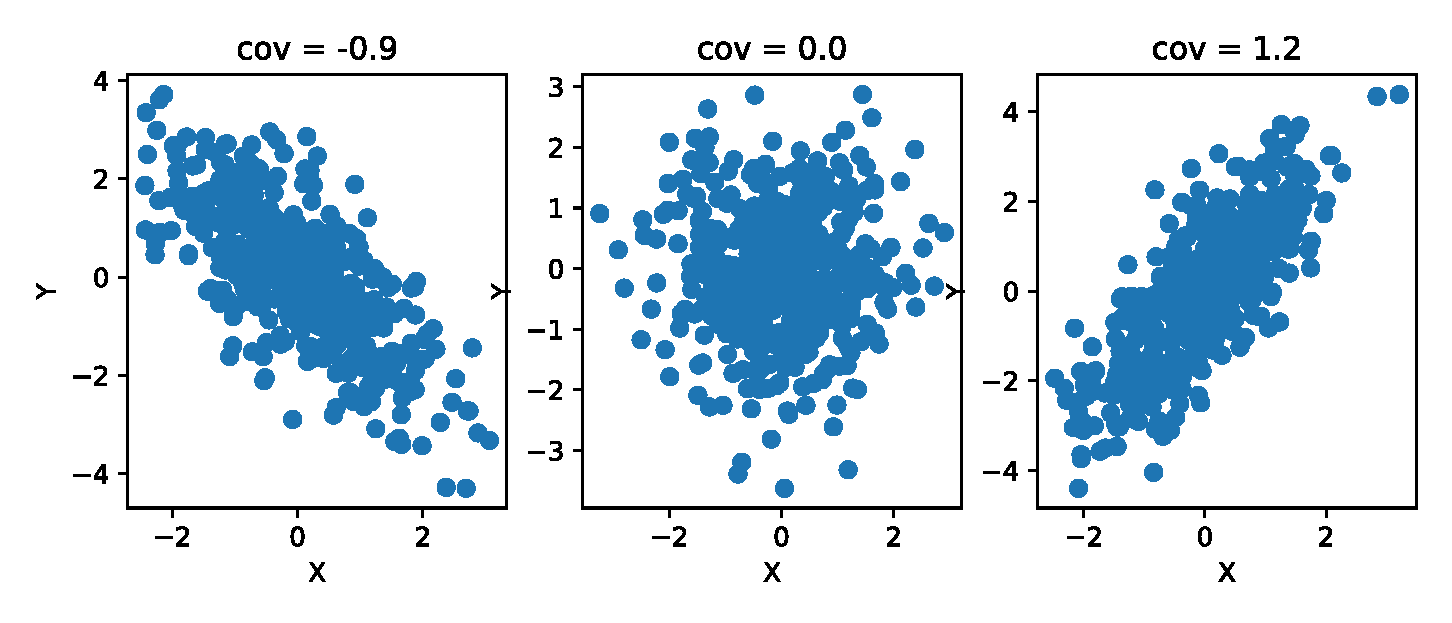
\includegraphics[width=0.6\textwidth]{fig/prob_cov.eps}
        \end{center}
    \end{frame}

    \begin{frame}
        Summarizing the main properties of covariance:
        \begin{itemize}
            \item For any RV $X$, $\mathrm{Cov}(X, X) = \mathrm{Var}(X)$
            \item For any RVs $X$ and $Y$ and numbers $a$ and $b$,
                  $\mathrm{Cov}(aX+b, Y) = \mathrm{Cov}(X, aY+b) = a\mathrm{Cov}(X, Y)$
            \item If $X$ and $Y$ are independent then $\mathrm{Cov}(X, Y) = 0$
        \end{itemize}

    \end{frame}

    \begin{frame}{Correlation}
        \vspace*{-2mm}
        \begin{boxed}
            \textbf{Correlation coefficient}:
            Define the \emph{correlation coefficient} to be
            $$\rho(X, Y) = \frac{\mathrm{Cov}(X, Y)}{\sigma_{X}\sigma_{Y}}$$
        \end{boxed}

        \vspace*{-1mm}
        Properties:
        \vspace*{-1mm}
        \begin{itemize}
            \item For any RV $X$, $\rho(X, X) = 1$
            \item For any RVs $X$ and $Y$ and numbers $a$ and $b$, $\rho(aX+b, Y) = \rho(X, aY+b) = \rho(X, Y)$
            \item If $X$ and $Y$ are independent with non-zero variance then $\rho(X, Y) = 0$
        \end{itemize}

        Visually:
        \vspace*{-5mm}
        \begin{center}
            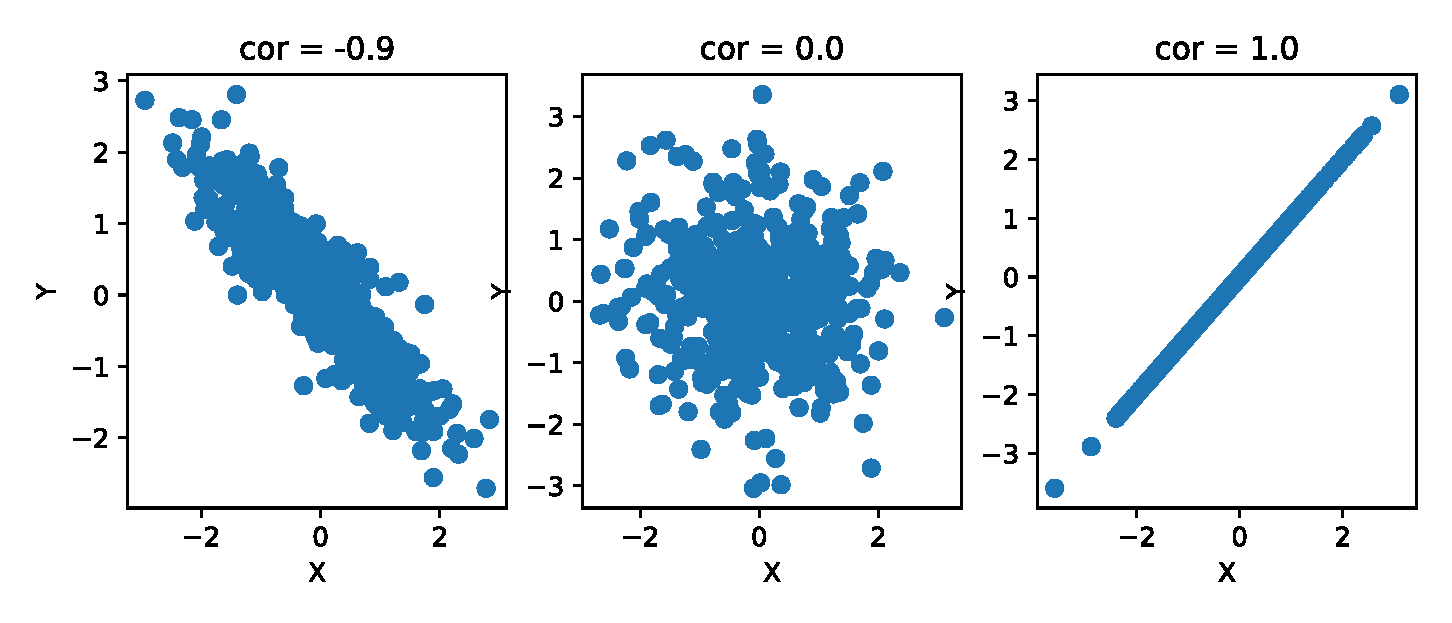
\includegraphics[width=0.6\textwidth]{fig/prob_corr.eps}
        \end{center}
    \end{frame}

    \begin{frame}{}
        \vspace*{2mm}
        \textbf{Example}\\[3mm]

        Let $X$ be any random variable, and $Y=aX+b$ as linear deterministic function of $X$.

        Then, one can compute that
        $$\sigma_{Y} = \sigma_{aX+b} = |a|\,\sigma_{X}$$

        $$\mathrm{Cov}(X, Y) = \mathrm{Cov}(X, aX+b) = a\mathrm{Cov}(X, X) = a\mathrm{Var}(X),$$

        and by definition

        $$\rho(X, Y) = \frac{a\mathrm{Var}(X)}{|a|\sigma_{X}^2} = \frac{a}{|a|} = \mathrm{sign}(a)$$

        Thus the correlation is $+1$ for any $a > 0$, and $-1$ for any $a < 0$.

        This shows that correlation
        measures the \emph{degree and directionality} of variation of the two RV, not the scale
        that the variation takes.
    \end{frame}

    % TODO
    % \begin{frame}{title}
    %     Show example: \url{http://d2l.ai/chapter_preliminaries/probability.html#an-example}
    %  \end{frame}

    \begin{frame}{Maximum Likelihood}

        Maximum Likelihood:
        \begin{itemize}
            \item A very common way of thinking in machine learning. Really it is a ``point of view''
            \item Given a probabilistic model with unknown parameters,
                  the most likely parameters are those under which the chance
                  that the model generated the data are maximized
        \end{itemize}

        Technically, given our data $X$, we want
        $$\hat{\boldsymbol{\theta}} = \arg \max_{\boldsymbol{\theta}} P(\boldsymbol{\theta}\mid X)$$
        where $\boldsymbol{\theta} = \mqty(\theta_1, \ldots, \theta_k)^\top$ the parameter vector
        of interest.

        Using Bayes' theorem the Maximum Likelihood Estimator (MLE) for $\boldsymbol{\theta}$ is
        $$\hat{\boldsymbol{\theta}}
            = \arg \max_{\boldsymbol{\theta}} \frac{P(X \mid \boldsymbol{\theta})P(\boldsymbol{\theta})}{P(X)}
            = \arg \max_{\boldsymbol{\theta}} P(X \mid \boldsymbol{\theta})P(\boldsymbol{\theta})$$
        since $P(X)$ is just scaling the objective w.r.t. $\boldsymbol{\theta}$.

        Exact same arguments apply to the densities of the continuous case.
    \end{frame}

    \begin{frame}{Maximum Likelihood: An Example}
        \begin{columns}[onlytextwidth]
            \begin{column}{0.7\textwidth}
                Setting:
                \begin{itemize}
                    \item Given a single, unknown parameter $\theta$: Probability that a coin flip is heads
                    \item Assume ``uniformative prior'' $\Rightarrow$ drop $P(\theta)$ from Bayes' theorem
                    \item Data: ``HHHTHTTHHHHHT'', i.e. $n_H = 9$ heads, $n_T = 4$ tails
                \end{itemize}
                \vspace*{3mm}

                Question: What is the probability that the coin comes up heads?\\
            \end{column}
            \begin{column}{0.3\textwidth}
                \begin{center}
                    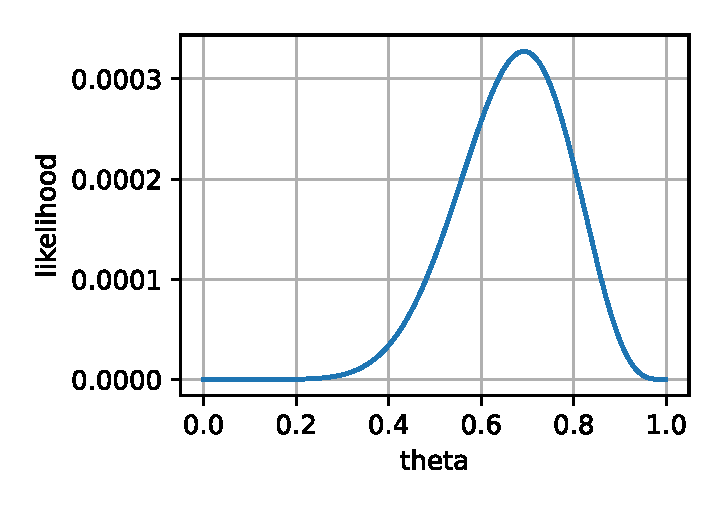
\includegraphics[width=\textwidth]{fig/prob_mle.eps}
                \end{center}
            \end{column}
        \end{columns}

        Answer: Assume samples independent $\Rightarrow$ probabilities multiply. Likelihood becomes
        $$P(X \mid \theta) = \theta^{n_H}(1-\theta)^{n_T} = P(X \mid \theta) = \theta^9(1-\theta)^4$$

        Then maximize the likelihood: The first-order condition
        $$
            \frac{d}{d\theta} P(X \mid \theta)
                = \frac{d}{d\theta} \theta^9(1-\theta)^4        
                = 9\theta^8(1-\theta)^4 - 4\theta^9(1-\theta)^3
                = \theta^8(1-\theta)^3(9-13\theta)
                = 0
        $$
        has three solutions: $0$, $1$ and $9/13$. First two are minima since
        $P(X\mid \theta=0) = P(X\mid \theta=1) = 0$. Last solution assigns non-zero probability
        to our data, hence the maximum likelihood estimate is $\hat \theta = 9/13.$\\
        {\tiny Note that despite everyone would correctly guess $9/13$, MLE provides
        a structured approach which equally applies to vastly more complex situations}

    \end{frame}

    \begin{frame}{Numerical Optimization and the Negative Log-Likelihood}
        In practice, we may have billions of parameters and examples.
        \begin{itemize}
            \item Independence assumption results in long product of small values, say, e.g.
                  $\prod_{i=1}^{10^9} \frac12$, something far below machine precision
            \item However, the $\log$ of this product is a sum,
                  $-\sum_{i=0}^{10^9} \log_{10} 2 = -10^9 \times \log_{10} 2 \approx -301029995.664$,
                  which fits into a 32-bit floating point value
        \end{itemize}

        Hence should work with log-likelihood,
        $$\log P(X \mid \boldsymbol{\theta})$$
        which will not affect the result since $\log$ is monotonically increasing.

        Often working with loss functions, to be \emph{minimized}, hence use negative log-likelihood:
        $$-\log P(X \mid \boldsymbol{\theta})$$

        Example: For the the coin flipping problem from before, this means minimizing
        $$-\log(P(X \mid \boldsymbol{\theta})) = -\log(\theta^{n_H}(1-\theta)^{n_T}) = -n_H\log(\theta) - n_T\log(1-\theta)$$
        which again leads to $\hat{\theta} = n_H/(n_H + n_T)$
    \end{frame}

    \subsection{Basic Distributions}

    \begin{frame}{Distributions}
        \framesubtitle{Bernoulli}
        Simple RV encoding e.g. a coin flip which comes up $1$ (heads)
        with probability $p$ and $0$ (tails) with probability $1-p$.

        \vspace*{3mm}
        \begin{columns}[onlytextwidth]
            \begin{column}{0.5\textwidth}
                \begin{boxed}
                    \textbf{Bernoulli Distribution}:
                    $$X \sim \mathrm{Bernoulli}(p) $$

                    Cumulative distribution function:
                    $$F(x) = \begin{cases} 0 & x < 0, \\ 1-p & 0 \le x < 1, \\ 1 & x \geq 1 . \end{cases}$$

                    Moments:
                    \begin{itemize}
                        \item  $\mu_X = p$
                        \item $\sigma_X^2 = p(1-p)$
                    \end{itemize}
                \end{boxed}
            \end{column}
            \begin{column}{0.5\textwidth}
                \begin{center}
                    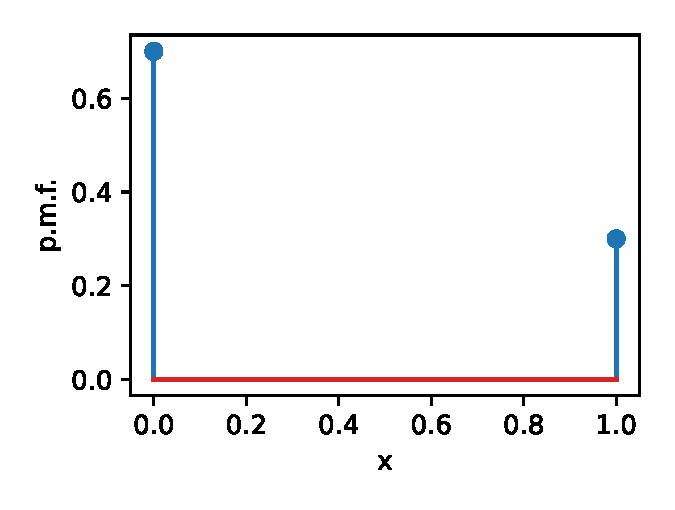
\includegraphics[width=0.8\textwidth]{fig/prob_dist_bernoulli.eps}
                \end{center}
            \end{column}
        \end{columns}
    \end{frame}

    \begin{frame}{Distributions}
        \framesubtitle{Discrete Uniform}
        Every value out of given set is equally likely has a probability of $p_i = \frac{1}{n}$ to occur

        \vspace*{3mm}
        \begin{columns}[onlytextwidth]
            \begin{column}{0.5\textwidth}
                \begin{boxed}
                    \textbf{Discrete Uniform Distribution}:
                    Assume the set of possible outcomes is $\{1, 2, \ldots, n\}$.
                    $$X \sim U(n)$$

                    Cumulative distribution function:
                    $$F(x) = \begin{cases} 0 & x < 1, \\ \frac{k}{n} & k \le x < k+1 \text{ with } 1 \le k < n, \\ 1 & x >= n . \end{cases}$$

                    Moments:
                    \begin{itemize}
                        \item $\mu_X = \frac{1+n}{2}$
                        \item $\sigma_X^2 = \frac{n^2-1}{12}$
                    \end{itemize}
                \end{boxed}
            \end{column}
            \begin{column}{0.5\textwidth}
                \begin{center}
                    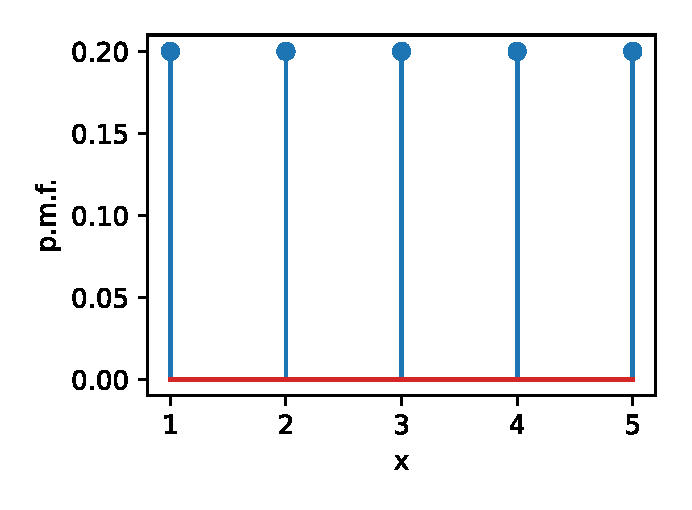
\includegraphics[width=0.8\textwidth]{fig/prob_dist_uniform.eps}
                \end{center}
            \end{column}
        \end{columns}
    \end{frame}

    \begin{frame}{Distributions}
        \framesubtitle{Continuous Uniform}
        \vspace*{-1mm}
        Similar to discrete uniform distribution: Starting from $U(n)$ with $n \rightarrow \infty$
        and linearly scaling it to the interval $[a,b]$ will approach a continuous random variable that just
        picks an arbitrary value in $[a,b]$ with equal probability

        \begin{columns}[onlytextwidth]
            \begin{column}{0.5\textwidth}
                \begin{boxed}
                    \textbf{Continuous Uniform Distribution}:
                    $$X \sim U(a, b)$$

                    $$\text{PDF:}\qquad p(x) = \begin{cases} \frac{1}{b-a} & x \in [a, b] \\ 0 & x \not\in [a, b]\end{cases}$$

                    $$\text{CDF:}\qquad F(x) = \begin{cases} 0 & x < a \\ \frac{x-a}{b-a} & x \in [a, b] \\ 1 & x >= b \end{cases}$$

                    $$\text{Moments:}\qquad \displaystyle \mu_X = \frac{a+b}{2} \quad \sigma_X^2 = \frac{(b-a)^2}{12}$$
                \end{boxed}
            \end{column}
            \begin{column}{0.5\textwidth}
                \begin{center}
                    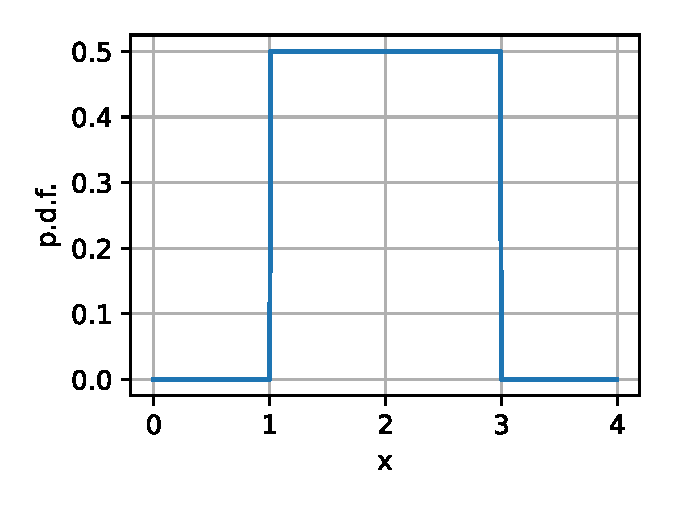
\includegraphics[width=0.55\textwidth]{fig/prob_cont_unif_pdf.eps}
                    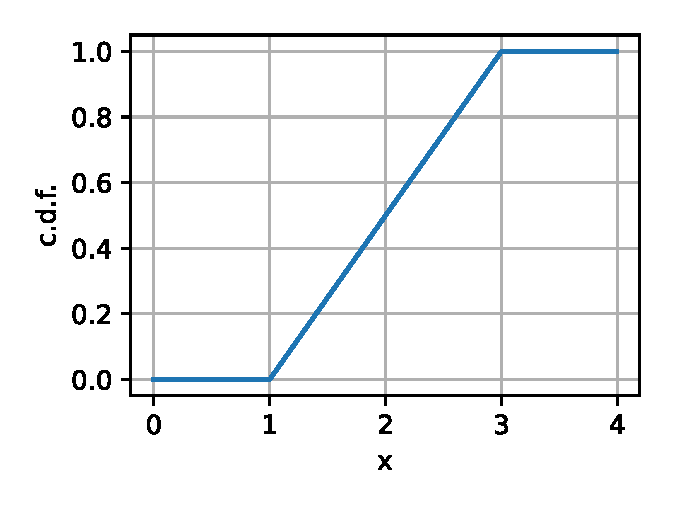
\includegraphics[width=0.55\textwidth]{fig/prob_cont_unif_cdf.eps}
                \end{center}
            \end{column}
        \end{columns}
    \end{frame}

    \begin{frame}{Distributions}
        \framesubtitle{Binomial}
        Given $n$ independent experiments, each with success probability $p$. Interested in
        number of successes $X$:
        $$X = \sum_{i=1}^n X_i \quad \text{with} \quad X_i \sim \mathrm{Bernoulli}(p)
            \qquad \Longleftrightarrow \qquad X \sim \mathrm{Binomial}(n, p)
        $$

        \vspace*{-2mm}
        \begin{boxed}
            \textbf{Binomial Distribution}:
            $$
                \text{CDF:}\qquad F(x) = \begin{cases}
                    0                                          & x < 0                                   \\
                    \sum_{m \le k} \binom{n}{m} p^m(1-p)^{n-m} & k \le x < k+1 \text{ with } 0 \le k < n \\
                    1                                          & x >= n
                \end{cases}
            $$

            $$\text{Moments:}\qquad \displaystyle \mu_X = np \quad \sigma_X^2 = np(1-p)$$
        \end{boxed}
        \vspace*{-3mm}
        \begin{center}
            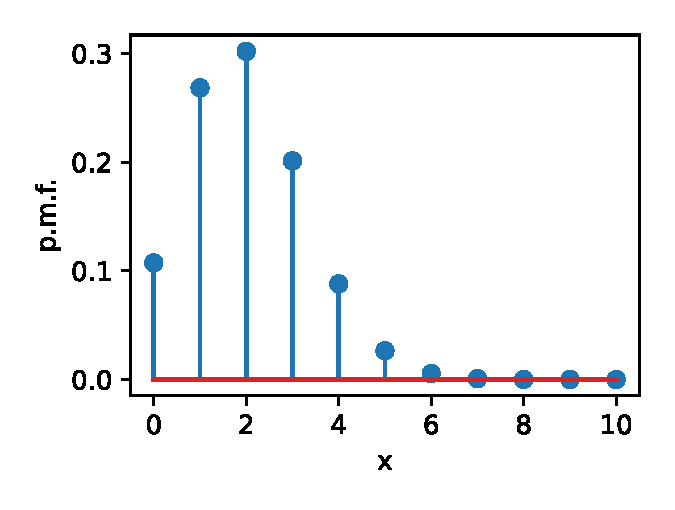
\includegraphics[width=0.3\textwidth]{fig/prob_binomial_pdf.eps}
            \qquad
            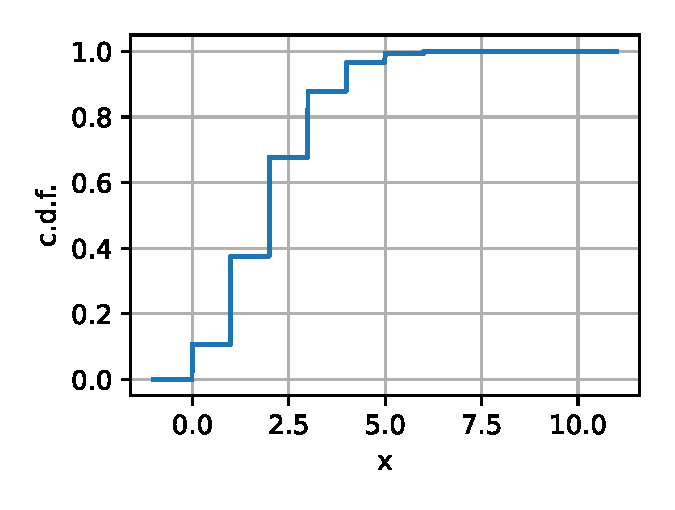
\includegraphics[width=0.3\textwidth]{fig/prob_binomial_cdf.eps}
        \end{center}

    \end{frame}

    \begin{frame}{Distributions}
        \framesubtitle{{Poisson}}
        \vspace*{-8mm}
        \begin{columns}[onlytextwidth]
            \begin{column}{0.57\textwidth}
                Model for arrival rates, e.g. number of buses at a given stop per
                time interval. Call this rate $\lambda$ (with units [1/s])
                \vspace*{2mm}

                \begin{boxed}
                    \textbf{Poisson Distribution}:
                    $$X \sim U(a, b)$$

                    $$\text{PMF:}\qquad p_k = \frac{\lambda^ke^{-\lambda}}{k!}$$

                    $$\text{CDF:}\qquad F(x) = \begin{cases} 0 & x < 0, \\ e^{-\lambda}\sum_{m = 0}^k \frac{\lambda^m}{m!} & k \le x < k+1 \text{ with } 0 \le k \end{cases}$$

                    $$\text{Moments:}\qquad \displaystyle \mu_X = \lambda \quad \sigma_X^2 = \lambda$$
                \end{boxed}
            \end{column}
            \begin{column}{0.43\textwidth}
                \begin{center}
                    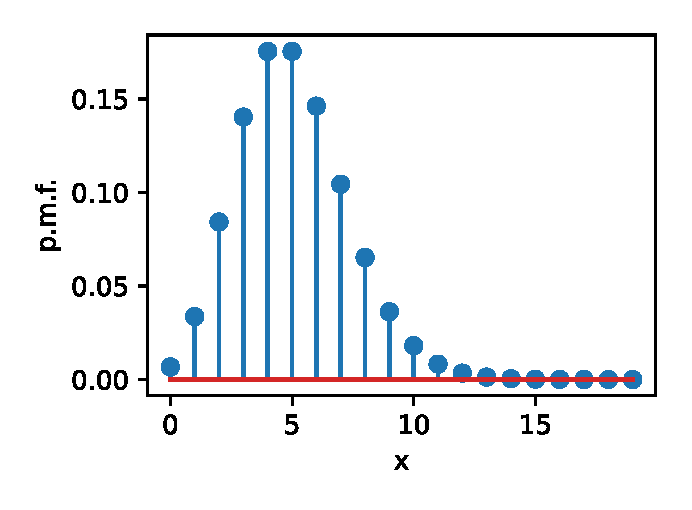
\includegraphics[width=0.8\textwidth]{fig/prob_poisson_pmf.eps}
                    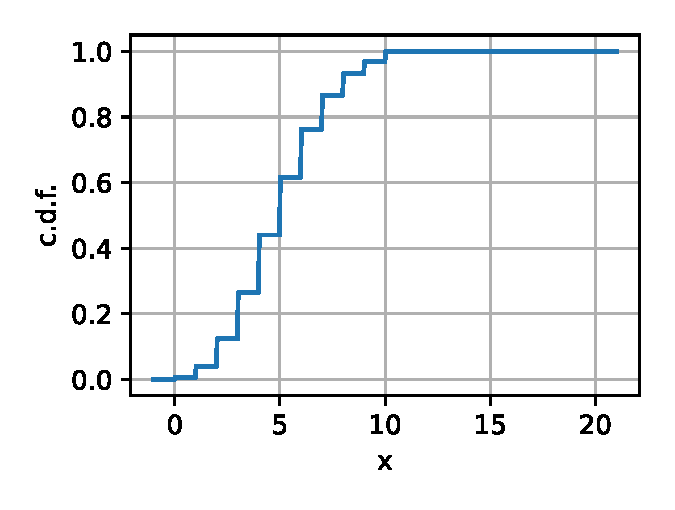
\includegraphics[width=0.8\textwidth]{fig/prob_poisson_cdf.eps}
                \end{center}
            \end{column}
        \end{columns}
    \end{frame}

    \begin{frame}{Distributions}
        \framesubtitle{Gaussian}

        \begin{columns}[onlytextwidth]
            \begin{column}{0.55\textwidth}
                The central distribution in probability theory with many unique properties because of
                the \emph{central limit theorem}.\\[1mm]

                Informally, given $N$ arbitrarily distributed, i.i.d. RVs $X_i$ and
                $$
                    X^{(N)} = \sum_{i=1}^N X_i
                $$
                their sum. Then, under mild conditions,
                $$
                    \frac{X^{(N)} - \mu_{X^{(N)}}}{\sigma_{X^{(N)}}} \quad \sim \quad \text{approximately Gaussian}
                $$

                \begin{boxed}
                    \textbf{Gaussian Distribution}:
                    $$X \sim \mathcal{N}(\mu, \sigma^2)$$
                    \vspace*{-2mm}
                    $$\text{PDF:}\qquad p_X(x) = \frac{1}{\sqrt{2\pi}\sigma}e^{-\frac{(x-\mu)^2}{2\sigma^2}}$$
                    $$\text{Moments:}\qquad \displaystyle \mu_X = \mu \quad \sigma_X^2 = \sigma^2$$
                \end{boxed}

            \end{column}
            \begin{column}{0.45\textwidth}
                \begin{center}
                    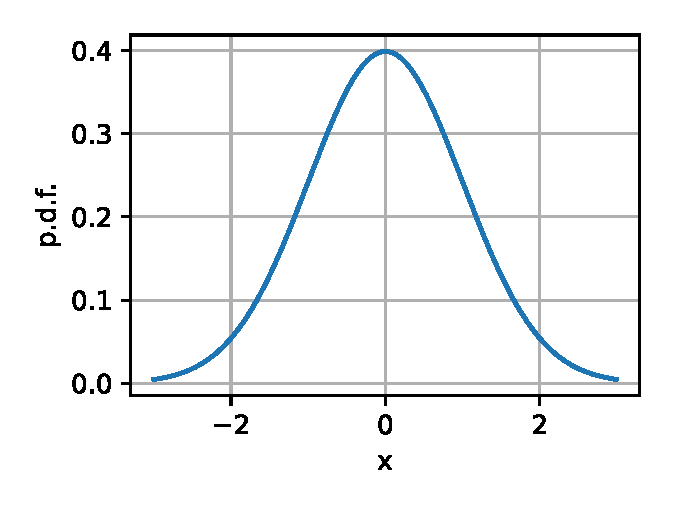
\includegraphics[width=0.73\textwidth]{fig/prob_norm_pdf.eps}
                    \qquad
                    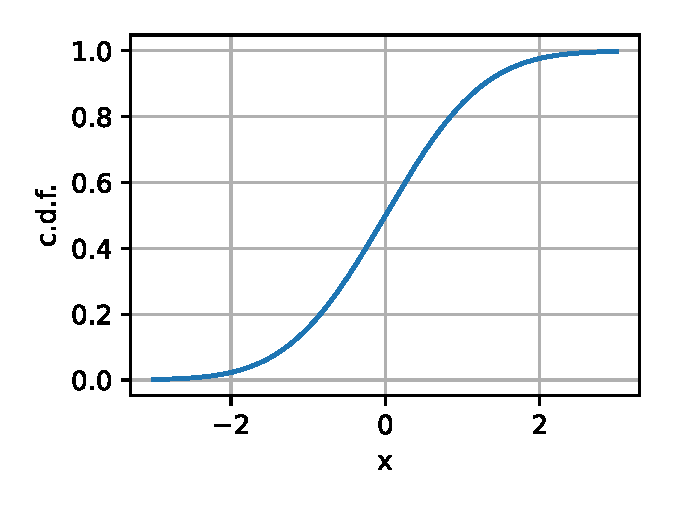
\includegraphics[width=0.73\textwidth]{fig/prob_norm_cdf.eps}
                \end{center}

            \end{column}
        \end{columns}
    \end{frame}


    \begin{frame}{Distributions: Summary}
        Things to remember about distributions:
        \begin{itemize}
            \item Bernoulli RVs can be used to model events with a yes/no outcome
            \item Discrete uniform distributions model selects from a finite set of possibilities
            \item Continuous uniform distributions select from an interval
            \item Binomial distributions model a series of Bernoulli RVs, and count the number of successes
            \item Poisson RVs model the arrival of rare events
            \item Gaussian RVs model the result of adding a large number of independent RVs together
            \item All the above distributions belong to the exponential family
        \end{itemize}
    \end{frame}

    % \begin{frame}{Statistics}
    %     probably should discuss this as well,
    %     \url{http://d2l.ai/chapter_appendix-mathematics-for-deep-learning/statistics.html}
    % \end{frame}
}